\documentclass[10pt]{article}
\usepackage[polish]{babel}
\usepackage[utf8]{inputenc}
\usepackage[T1]{fontenc}
\usepackage{graphicx}
\usepackage[export]{adjustbox}
\graphicspath{ {./images/} }
\usepackage{amsmath}
\usepackage{amsfonts}
\usepackage{amssymb}
\usepackage[version=4]{mhchem}
\usepackage{stmaryrd}

\title{Zestaw 2 }

\author{}
\date{}


\begin{document}
\maketitle
\section*{KLASY PIERWSZE I DRUGIE}
\begin{enumerate}
  \item Pierwszą cyfrą liczby 6-cyfrowej jest 3. Jeżeli tę cyfrę przesuniemy z pierwszego miejsca na ostatnie, to otrzymamy czwartą część pierwszej liczby. Co to za liczba?
  \item Zapalono dwie świece o różnych długośsiach i grubościach. Dłuższa z nich spala się zupełnie w ciągu 3 godzin, krótsza w ciągu 5 godzin. Po dwóch godzinach palenia długości obu świec wyrównały się. Ile razy jedna świeca była dłuższa od drugiej przed zapaleniem?
  \item Dwa trójkąty równoboczne o obwodach 17 i 19 są położone jak na rysunku (ich boki są parami równoległe). Oblicz obwód sześciokąta, którego wierzchołki są punktami przecięcia boków trójkąta.\\
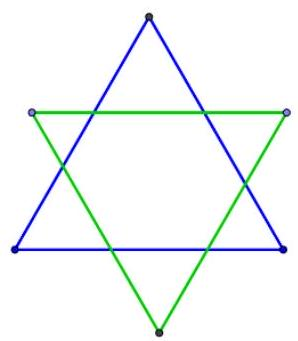
\includegraphics[max width=\textwidth, center]{2024_11_21_2afe1455fa3bbe8bb7f8g-1}
\end{enumerate}

\section*{KLASY TRZECIE I CZWARTE}
\begin{enumerate}
  \item Niech \(p\) będzie dowolną liczbą pierwszą. Udowodnij, że reszta z dzielenia liczby \(p\) przez 30 nie jest liczbą złożoną .
  \item Dany jest sześcian o krawędzi \(a\). Oblicz promień kuli stycznej do kuli wpisanej w ten sześcian i do trzech ścian sześcianu.
  \item Dla jakich wartości parametru \(m\) nierówność
\end{enumerate}

\[
\left(m^{2}-1\right) \cdot 25^{x}-2(m-1) \cdot 5^{x}+2>0
\]

jest spełniona przez każdą liczbę rzeczywistą x?


\end{document}